\documentclass[a4paper, titlepage]{article}
\usepackage{graphicx}
\usepackage{biblatex}
\usepackage{parskip}
\usepackage{multicol}
\usepackage{listings}
\usepackage{xcolor}

\lstset{
  basicstyle=\ttfamily,
  columns=fullflexible,
  breaklines=true,
  postbreak=\raisebox{0ex}[0ex][0ex]{\color{red}$\hookrightarrow$\space}
}

\graphicspath{ {./Images/} }
\addbibresource{biblography.bib}
\setcounter{tocdepth}{4}

\title{Parser Documentation}
\author{Adam Rehman, Brandon Cann, Xin Wang \thanks{document compiled by Xin Wang}}
\date \today
\date{\today}

\setlength{\parskip}{1em}

\begin{document}
    \maketitle
    
    \tableofcontents
    \pagebreak
 
    \section{Introduction}
    \indent
    Based on the provided project briefing, a netlist describing the circuit will be provided in a file 
    using a reduced SPICE format. It is required by the team to formulate an approach to reading the input format and 
    store the information in a comprehensible and efficient data structure. 
    \par
    This document will research the format of the SPICE netlist and explore the different approaches in 
    storing the information a certain way. 
    \vfill
    \begin{center}
        \textit{This document is primarily used for planning the most effective 
        way to approach the problem as well as allowing fellow teammates to 
        engage productively on a equal knowledge footing.}
    \end{center}
    \pagebreak
    \section{Input (.cir) file}
    Source file for any version of SPICE has the following format \cite{spice}.
    \begin{quotation}
        {\fontfamily{qcr}\selectfont
            title \par
            elements \par
            .model statements \par
            analysis commands \par
            output commands \par
            .end \par
        }
    \end{quotation}

    \begin{figure}[h]
        \centering
        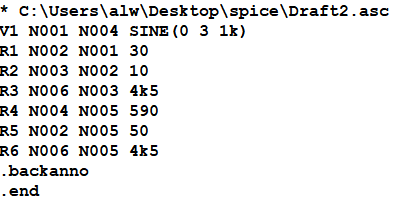
\includegraphics[width=60mm,scale=1]{spice netlist example}
        \caption{Netlist input example}
        \label{fig:Netlist input example}
    \end{figure}

    \textbf{Important points to note:}
    \begin{itemize}
        \item First line {\fontfamily{qcr}\selectfont title } is used as a title on output files.
        \begin{itemize}
            \item Parser ignores the first line of the netlist.
        \end{itemize}
        \item File must end with command {\fontfamily{qcr}\selectfont .end}.
        \begin{itemize}
            \item Parser exits when {\fontfamily{qcr}\selectfont .end} is encountered.
        \end{itemize}
        \item Comment begins with '*' which covers entire line.
        \begin{itemize}
            \item Parser ignores entire line if a '*' char is at the beginning.
        \end{itemize}
    \end{itemize}
    \pagebreak
    \section{Netlist Element Format}
    A \textbf{netlist} will contain a set of statements defining elements in a circuit.
    \par
    Connections are described by naming nodes. The program will automatically assign a number to the nodes in the circuit
    starting from 1. 
    \par
    \textbf{Node 0 is defined as Ground}. It is necessary to have a Node 0 since it is the reference point for 
    all voltages specified.
    \par
    Initial stage of the parser will only be able to support input with nodes starting from N1 and ground defined as N0.
    SPICE defined ground node as $0$. Suport for complex values such as 4k5 will be added at a later stage too.
    This will be revised when basic function of Analysis module is implemented.
    \par
    We have to consider a situation where the input syntax is correct but the circuit represented is unrealizable.
    To overcome this, we will need a function to check if the circuit described is realistic. This is explored more
    in the $Analysis$ module.

    \subsection{Basic components}
    Current supported elements are basic passive elements. \par
    Passive elements are composed of the following:\footnote{Initial conditions for C and L are optional and default set to 0}
    \begin{itemize}
        \item Resistors: {\fontfamily{qcr}\selectfont R} $$ \tt R<description> <n1> <n2> <value> $$
        \item Capacitor: {\fontfamily{qcr}\selectfont C}. $$ \tt C<description> <n1> <n2> <value><initial-condition>$$ 
        \item Inductor: {\fontfamily{qcr}\selectfont L}. $$ \tt L<description> <n1> <n2> <value><initial-condition>$$ 
    \end{itemize}
    Both $C$ and $L$ will be considered at a later stage. First versions implemented will cover resistors only. This
    approach will allow the core functionalities of the program to be consolidated and, with the experience gained, 
    will allow us to find the best approach to implement more complex functions.
    \vfill
    \pagebreak
    \subsection{Independent Sources}
    The character after the letter must be a unique instance name.
    \subsubsection{Independent DC sources}
    \begin{itemize}
        \item Voltage Sources: 
        \begin{center}
            $\tt V<description> <n+> <n-><value>$
        \end{center}
        \item Current Sources:
        \begin{center}
            $\tt I<description> <n+> <n-><value>$
        \end{center}
    \end{itemize}
    \subsubsection{Independent $Sine$ sources}
    \begin{itemize}
        \item Voltage Sources: 
        \begin{center}
            $\tt V<description> <n+> <n->SINE<Offset><Amplitude><Frequency>$
        \end{center}
        \item Current Sources:
        \begin{center}
            $\tt I<description> <n+> <n->SINE<Offset><Amplitude><Frequency>$
        \end{center}
    \end{itemize}
    \textbf {When users are entering component values, it is important that the software recognises common abbreviations 
    for units.}
    \subsubsection{Diode}
    \subsection{Analysis functions}
    \subsubsection{.tran function}
    \begin{center}
        $\tt .tran <tstep><tstop> <tstart <tmax>>$
    \end{center}


    \pagebreak
    \subsection{Support for powers of ten}
    In order to support {\fontfamily{qcr}\selectfont spice} format, the following abbreviations for powers of ten 
    must be recognised and are case sensitive:
    \begin{multicols}{2}
    \begin{itemize}
        \item f [femto]: $ 10^{-15} $
        \item p [pico]: $ 10^{-12} $
        \item n [nano]: $ 10^{-9} $
        \item u [micro]: $ 10^{-6} $
        \item m [milli]: $ 10^{-3} $
        \item k [kilo]: $ 10^{+3} $
        \item Meg [mega]: $ 10^{+6} $
        \item g [giga]: $ 10^{+9} $
        \item t [tera]: $ 10^{+12} $
    \end{itemize}
    \end{multicols}
    Any unrecognised characters are ignored.
    
    \pagebreak
    \section{Network Diagram/Graphs}
    Network Graphs show the relationships between a set of entries and a circuit is a good example of a graph.
    Each entry is represented by a \textit{Node} and the connections between nodes are represented through \textit{Edges}.
    \par
    Through Modified Nodal Analysis, an algorithm can be created to form the expression $Ax = b$.
    \par
    The circuit inputted will be in vector of nodes which will then be read and inputted into the required matrices.

    \par
    This will be explored further in the analysis module.
    \pagebreak

    \section{Implementation}
    Block diagram depicting the breakdown of Parse Netlist module:
    \begin{center}
        \begin{figure}[h]
        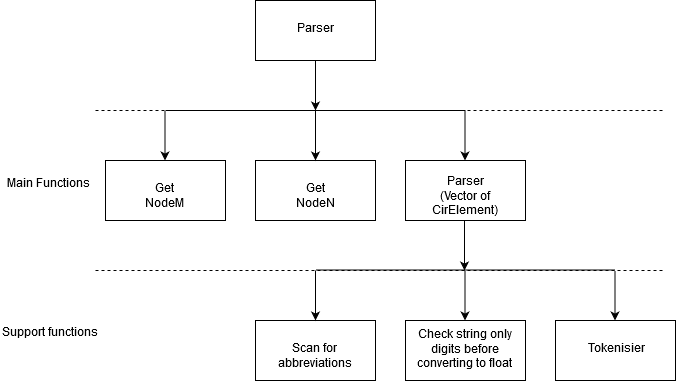
\includegraphics[width=\linewidth]{Netlist breakdown}
        \caption{Netlist module breakdown}
        \label{fig:Netlist breakdown}
        \end{figure}
    \end{center}
    
    \subsection{CirElement struct}
    \begin{lstlisting}[language=C++]
        struct CirElement 
        {
            letter: component name
            name: name of node
            node1: node this node is connected to 
            node2: node this node is connected to
            value: float
        }

        struct CirSrc
        {
            letter: component name
            name: name of node
            node1: node this node is connected to 
            node2: node this node is connected to
            type: string: DEFAULT "DC"
            DC: float
            A: float
            freq: float
        }
    \end{lstlisting}
    \subsection{Parser}
    \begin{lstlisting}[language=C++]
        parser(cin, &vector<CirElement>, &vector<CirSrc>)
        {
            Tokenise
            Put in values into respective variables
                if 'v' or 'i' detected:
                    Call SrcSort
                if other elements detected:
                    Push into CirElement
                Detect values, pass into custom_pow
                Push CirElement into vector
        }
    \end{lstlisting}
    \subsubsection{converter}
    Basic function: e.g. 5k, 50 etc
    \begin{lstlisting}[language=C++]
        converter(string: input)
        {
            Check if there are keywords e.g. k, m, M, G
    
            If not present, two scenario:
                Unknown letter present: extract digits 
                Convert to float
                Empty string (End of recursion): return 0
    
            If present:
                Find position where keyword appears
                Take string before keyword and convert
                Multiply/divide the digit by keyword
        }
    \end{lstlisting}

    \subsubsection{tokeniser}
    \begin{lstlisting}[language=C++]
        tokeniser(string: input)
        {
            Call regex to tokenise the string 
            Push each token into a vector 
            Return vector
        }
    \end{lstlisting}

    \subsubsection{isdigit}
    \begin{lstlisting}[language=C++]
        isdigit(string: input)
        {
            Iterate over string
            Take each character and into 'isdigit' test
            Return boolean
        }
    \end{lstlisting}
    \subsection{Node N}
    \begin{lstlisting}[language=C++]
        getnodeN(vector<CirElement>: input)
        {
            Return size of vector<CirElement>
        }
    \end{lstlisting}
    \subsection{Node M}
    \begin{lstlisting}[language=C++]
        getnodeM(vector<CirSrc>)
        {
            Return size of vector<CirSrc>
        }
    \end{lstlisting}
    \pagebreak
    \section{Version history}
    \subsection{Version 1.0}
    Basic functionality of the Parser is implemented.
    \subsubsection{List of functions}
    \begin{itemize}
        \item Basic circuit components recognised.
    \end{itemize}
    \subsubsection{Still to do for v2.0}
    \begin{itemize}
        \item Recognise SINE voltage source.
        \item Recognise grounded nodes appear as $0$ only.
        \item Recognise transient function calls.
    \end{itemize}

    \pagebreak
    \section{Add-ons}
    There are more components to consider such as:
    \begin{itemize}
        \item Voltage controlled dependent sources
        \item Current controlled dependent sources
        \item Diodes
        \item BJT
        \item MOSFET
        \item Python implementation
        \item Efficient way to use recursion and not efficient to use matrix but more accurate.
    \end{itemize}
    
    \pagebreak
    \printbibliography[title={References}]

\end{document}